\documentclass[18pt]{beamer}

\usetheme{Madrid} % [secheader]
\setbeamertemplate{footline}{}
\usefonttheme{professionalfonts}
\usepackage[english]{babel}
\usepackage{graphicx}
\usepackage[normalem]{ulem}
\usepackage{hyperref}
\usepackage{bm}
\usepackage{dsfont}
\usepackage{subcaption}
\usepackage{natbib}
\usepackage{bbm}
\usepackage{calc}  % For widthof command
\usepackage{xcolor}
\usepackage{natbib}
\bibliographystyle{abbrvnat}
\setcitestyle{authoryear, open={(}, close={)}}

\setbeamerfont{itemize/enumerate subbody}{size=\normalsize} %to set the body size
%\setbeamertemplate{frametitle}[default][center]
\setbeamertemplate{itemize subitem}{\normalsize\raise1.25pt\hbox{\donotcoloroutermaths$\blacktriangleright$}}  %to set the symbol size

% HMC related macros
\newcommand{\position}{\theta}
\newcommand{\momentum}{p}
\newcommand{\bposition}{\bm{\position}}
\newcommand{\bmomentum}{\bm{\momentum}}
\newcommand{\Position}{\Theta}
\newcommand{\Momentum}{P}
\newcommand{\integrationTime}{\tau}
\newcommand{\pathlen}{L}
\newcommand{\stepsize}{\Delta t}
\newcommand{\solutionOp}{\bm{\Psi}}
\newcommand{\involution}{\bm{R}}

% Math macros
\newcommand{\transpose}{\text{\raisebox{.5ex}{$\intercal$}}}
\newcommand{\diff}{{\rm d}}
\newcommand{\Diff}{\mathbf{D}}

% Probability / statistics macros
\newcommand{\given}{\, | \,}
\newcommand{\normal}{\mathcal{N}}
\newcommand{\proposalKernel}{Q}

% Variable / Greek symbol macros
\newcommand{\y}{\bm{y}}
\newcommand{\x}{\bm{x}}
\newcommand{\I}{\bm{I}}
\newcommand{\bPhi}{\bm{\Phi}}
\newcommand{\bSigma}{\bm{\Sigma}}
\newcommand{\nparam}{d}

% Utility macros
\newcommand{\todo}[1]{\textcolor{red}{#1}}

% Custom environments
\newcommand{\defineWithinItemizeSpacing}{
	\setlength{\abovedisplayskip}{.3\baselineskip}
	\setlength{\belowdisplayskip}{.3\baselineskip}
}
\newenvironment{itemizedEquation}{
	\defineWithinItemizeSpacing
	\begin{equation}
}{
	\end{equation} \ignorespacesafterend
}
\makeatletter
\newenvironment{itemizedEquation*}{
	\defineWithinItemizeSpacing
	\begin{equation*}
}{
	\end{equation*} \ignorespacesafterend
}
\makeatother


% Color definitions
\definecolor{uclablue}{RGB}{39, 116, 174}
\definecolor{navyblue}{rgb}{0.0, 0.0, 0.5}
\definecolor{turquoise}{rgb}{0.19, 0.84, 0.78}
\definecolor{mediumturquoise}{rgb}{0.28, 0.82, 0.8}
\definecolor{lava}{rgb}{0.81, 0.06, 0.13}

% Set the color theme of the presentation
\usecolortheme[named=uclablue]{structure}
\colorlet{textcolor}{white}
\setbeamercolor{frametitle}{fg=textcolor}
\setbeamercolor{titlelike}{fg=textcolor}
\setbeamercolor{section in head/foot}{fg=textcolor}
%\colorlet{toccolor}{black}
%\setbeamercolor{section in toc}{fg=toccolor}

%  Block colors
\setbeamercolor{block title}{use=structure, fg=textcolor, bg=structure.fg}
\setbeamercolor{block body}{
	parent=normal text, use=block title, bg=block title.bg!10}
%\setbeamercolor{block title}{bg=uclablue!100, fg=white}


\setbeamertemplate{enumerate items}[default]
\setbeamerfont*{itemize/enumerate body}{size=\normalsize}
\setbeamerfont*{itemize/enumerate subbody}{parent=itemize/enumerate body}
\setbeamerfont*{itemize/enumerate subsubbody}{parent=itemize/enumerate body}

\setbeamercovered{dynamic}
\setbeamercovered{invisible}
\beamertemplatenavigationsymbolsempty

% Insert table of content frames between sections automatically. See http://en.wikibooks.org/wiki/LaTeX/Presentations
\AtBeginSection[]
{
  \begin{frame}
    \frametitle{Table of Contents}
    \tableofcontents[currentsection]
    %    \tableofcontents[currentsection, currentsubsection]
  \end{frame}
}

\title[Bayesian Sparse GLM]{Practical introduction to Hamiltonian Monte Carlo}
\author{Aki Nishimura\inst{1}}
\institute[]{Department of Biomathematics, University of California - Los Angeles \inst{1}}
\date{\today}


\begin{document}
\frame{\titlepage}


\section{Why \& What to learn about Hamiltonian Monte Carlo}

\frame{
	\frametitle{What is Hamiltonian Monte Carlo (HMC)?}
	\begin{itemize}
	\item HMC is a state-of-the-art \textit{general-purpose} sampler, only requiring evaluation of the target log-density and its gradient.
	\item Required computations can be done algorithmically and efficiently for probabilistic models (or, more precisely, Bayesian networks):
		\begin{itemize}
		\item density evaluation via \textit{computational (directed acyclic) graphs} 
		\item gradient via \textit{reverse mode differentiation} / \textit{back-propagation}
		\end{itemize}
	\begin{figure}
		\centering
		\hspace{-.1\linewidth}
		
\includegraphics[height=.45\textheight]{Figure/probabilistic_programming_languages}
	\end{figure}
	\end{itemize}
}

\frame{
	\frametitle{What is HMC? (and what it is \textbf{not})}
	\begin{itemize}
	\item HMC is \textbf{not} a silver-bullet, though often good enough for computing posteriors of not-overly-complicated models with moderate sized data.
	\item HMC can be almost guaranteed to fail on certain target distributions.
		\begin{itemize}
		\item Work-arounds may exists in some cases, but not always.
		\end{itemize}
	\item Performance of HMC is sensitive to
		\begin{itemize}
		\item parametrization of the model.
		\item tuning parameters (which may be adjusted during a ``warm-up'').
		\end{itemize}
	\item In general, prefer
		\vspace{-.75\baselineskip}
		\begin{multline*}
		\text{model-specific inference algorithm by an expert} \\
			> \text{probabilistic programming implemnetation} \\
			> \text{your own code} \hspace{.05\linewidth}
		\end{multline*} \vspace{-1.5\baselineskip}
	\item When no other solid solutions exists, use Bayesian modeling and posterior computation via HMC as ``the least of all possible evils.''
	\end{itemize}
}

\frame{
	\frametitle{What is HMC? (and what it is \textbf{not})}
	\begin{itemize}
	\item Some softwares (e.g.\ \texttt{rstanarm}) incorporate model-specific best practices in applying HMC, yielding quite impressive performance.
	\item Some cutting-edge Bayesian methods rely on HMC for posterior computation with competitive computational efficiency.
		\begin{itemize}
		\item e.g.\ Bayesian sparse regression for GLM and survival analysis
		\end{itemize}
	\end{itemize}
}

\frame{
	\frametitle{Learning objectives: things to take home with}
	\begin{itemize}
	\item Sensitivity of HMC's performance means that, even as an end-user, one benefits from basic understandings of the algorithm.
	\item Hopefully, you will 
		\begin{itemize}
		\item know how to parametrize your model for best HMC performance.
		\item develop intuitions as to when posterior computation is feasible.
		\item be able to diagnose (and fix if possible) when sampling fails.
		\item know when to change default parameters in software packages.
		\item be familiar with research frontiers and improvements on the way.
		\end{itemize}
	\end{itemize}
}


\section{History and Motivation behind HMC}

\frame{
	\frametitle{History of ``H''MC}
	\begin{itemize}
	\item Invented as "hybrid" Monte Carlo in computational physics literature for computer simulation of lattice models in quantum field theory.
	\item At the time, there were two dominant approaches:
		\begin{itemize}
		\item Monte Carlo simulation based on "local" moves, changing the state of one particle at a time.
		\item molecular dynamics simulation with "global" moves by numerically solving \textit{equations of motion}.
		\end{itemize}
	\item "Hybrid" Monte Carlo combined the efficiency of molecular dynamics with Metropolis algorithm to ensure the exact stationary distribution.
	\end{itemize}
}

\frame{
	\frametitle{What does Hamiltonian dynamics have to do with MCMC?}
	\begin{itemize}
	\item Two (often competing) objectives in constructing a proposal density:
		\begin{itemize}
		\item you want to make "large" moves to explore the space. 
		\item you want sufficiently high acceptance rates.
		\end{itemize}
	\item e.g.\ random-walk Metropolis for $\nparam$-dimensional Gaussians:
		\begin{itemize}
		\item Proposal variance needs to be $O\big(d^{-1}\big)$ for $O(1)$ acceptance rate.
		\item It takes $\nparam$ steps for the chain to travel $O(1)$ distance.
		\item The cost of generating one effective sample is proportional to
			\begin{itemizedEquation*}
			\nparam \times \text{(cost of likelihood evaluation)}. 
			\end{itemizedEquation*}
		\item Note: the cost is often described as $O(d^2)$ in the literature.
		\end{itemize}
	\item Question: can we generate proposals that are far away from the current state, yet still maintains high acceptance rate? 
		\begin{itemize}
		\item Yes, use Hamiiltonian dynamics to generate proposals! 
		\item In particular, HMC has the cost of $O(d^{1 / 4})$ in the above example.
		\end{itemize}
	\end{itemize}
}


\section{Title TBD}

\frame{
	\frametitle{Set-up and terminologies for HMC}	
	\begin{itemize}
		\item To sample from the distribution of interest $\pi_\Position(\bposition)$, HMC augments the parameter space with an auxiliary parameter $\bmomentum \in \mathbb{R}^\nparam \sim \normal(\mathbf{0}, m \I)$.
		\item HMC then samples from the joint density
		\begin{itemizedEquation*}
		\pi(\bposition, \bmomentum) 
			\propto \pi_\Position(\bposition) \times \mathcal{N}\left( \bmomentum \, ; \mathbf{0}, m \I \right) 
		\end{itemizedEquation*}
		where $\bposition$ and $\bmomentum$ are referred to as \textit{position} and \textit{momentum} variables.
		\item HMC terminologies:
		\begin{itemize}
			\item $U(\bposition) = - \log \pi_\Theta(\bposition)$ : \textit{potential energy}.
			\item $K(\bmomentum) = \frac{1}{m} \bmomentum^\transpose \bmomentum$ : \textit{kinetic energy}.
			\item $H(\bposition, \bmomentum) = U(\bposition) + K(\bmomentum) = - \log \pi(\bposition, \bmomentum)$ : \newline \phantom{$H(\bposition, \bmomentum) = U(\bposition) + K(\bmomentum)$ =} \textit{Hamiltonian} or \textit{total energy}.
		\end{itemize}
	\end{itemize}
}

\frame{
	\frametitle{Transition kernel of HMC}
	\begin{itemize}
	\item HMC generates a proposal by combining momentum randomization and \textit{deterministic} transition of simulated Hamiltonian dynamics.
	\end{itemize}
	\begin{block}{HMC transition rule}
		Given the current state $(\bposition_0, \bmomentum_0)$, HMC generates the next state as follows:
		\begin{enumerate}
			\item Randomize momentum: $\bmomentum_0 \sim \mathcal{N}\left(\mathbf{0}, m \I \right)$.
			\item Generate a proposal $(\bposition^*, \bmomentum^*) \approx (\bposition(\integrationTime), - \bmomentum(\integrationTime))$ by approximating \newline the solution $\left\{ (\bposition(t), \bmomentum(t)) : t \in [0, \integrationTime] \right\}$ of \textit{Hamilton's equation}
				\vspace{-.3\baselineskip}
				\begin{equation} \label{eq:hamilton}
				\vspace{-.3\baselineskip}
				\begin{aligned}
				\frac{\diff \bposition}{\diff t} 
				&= m^{-1} \bmomentum, \quad
				\frac{\diff \bmomentum}{\diff t} 
				= - \nabla_{\bposition} U(\bposition) 
				\end{aligned}
				\end{equation}
				with initial condition $(\bposition(0), \bmomentum(0)) = (\bposition_0, \bmomentum_0)$.
			\item Accept or reject the proposal. 
				% with the probability $$ \min\left\{1, \pi(\bposition^*, \bmomentum^*) / \pi(\bposition, \bmomentum) \right\} $$
		\end{enumerate}
	\end{block}
}

\frame{
	\frametitle{Physical interpretation of HMC trajectories}
	\begin{itemize}
	\item Hamilton's equation describes a motion of a particle with mass $m$ under the potential energy field $U(\bposition)$:
		\begin{itemizedEquation*}
		\begin{aligned}
		\text{``velolicty''}
			&= \frac{\diff \bposition}{\diff t} 
			= m^{-1} \bmomentum
			\\
		\text{``mass $\times$ acceleration''}
			&= \frac{\diff \bmomentum}{\diff t} 
			= - \nabla_{\bposition} U(\bposition) 
			= \text{``force''}
		\end{aligned}
		\end{itemizedEquation*}
	\item Trajectory $\bposition(t)$ accelerates toward lower values of the potential $U(\bposition)$ or, equivalently, larger values of $\log \pi_\Position(\bposition) = - U(\bposition)$.
	\end{itemize}
}

\frame{
	\frametitle{Visual illustration: HMC in action}
	\begin{center}
	\href{run:Figure/hmc_in_action_2d_Gaussian.avi}{\color{mediumturquoise} \fontsize{16pt}{18pt} \selectfont HMC for a 2d Gaussian (correlation $= 0.9$)}
	\vspace{4ex}

	\href{run:Figure/hmc_in_action_2d_Gaussian_slow_motion.avi}{\color{mediumturquoise} \fontsize{16pt}{18pt} \selectfont Click here for slow motion version}
	\end{center}
}


\section{Theory of HMC: exactness (at stationarity) \& high acceptance rates}

\frame{
	\frametitle{HMC as a valid Metropolis algorithm}
	\begin{itemize}
	\item Hamiltonian dynamics generates a \textit{symmetric} proposal 
	\begin{itemizedEquation*}
	\proposalKernel\left\{ (\bposition, \bmomentum) \to (\bposition^*, \bmomentum^*)  \right\}
		= \proposalKernel\left\{ (\bposition^*, \bmomentum^*) \to (\bposition, \bmomentum) \right\}
	\end{itemizedEquation*}
	by virtue of its \textit{reversibility} (and \textit{volume-preservation}).
		\begin{itemize}
		\item For a deterministic proposal kernel, interpret the symmetry as
		\begin{itemizedEquation*}
		\proposalKernel\left\{ S \to S^* \right\}
			= \proposalKernel\left\{ S^* \to S \right\}
		\end{itemizedEquation*}
		for a pair of sets $S$ and $S^*$.
		\end{itemize}
	\item Evolution of Hamiltonian dynamics can be ``reversed'' (or ``inverted'') by flipping momentum and applying the same dynamics:
		\begin{itemizedEquation*}
		(\bposition, \bmomentum) \to (\bposition', \bmomentum')
			\quad \Leftrightarrow \quad
			(\bposition', -\bmomentum') \to (\bposition, -\bmomentum)
		\end{itemizedEquation*}
	\end{itemize}
}

\frame{
	\frametitle{Symmetry via reversibility of Hamiltonian dynamics}
	\begin{itemize}
	\item Let $\{ \solutionOp_t \}_{t \in \mathbb{R}}$ denote the \textit{solution operator} of dynamics i.e.\ 
		\begin{itemizedEquation*}
		(\bposition(t), \bmomentum(t)) := \solutionOp_t(\bposition, \bmomentum)
		\end{itemizedEquation*}
		solves Hamilton's equations and $\solutionOp_0(\bposition, \bmomentum) = (\bposition, \bmomentum)$.
	\item Let $\involution(\bposition, \bmomentum) = (\bposition, - \bmomentum)$ denote the momentum flip operator.	
	\item \textit{Reversibility} of dynamics means that
		\begin{itemizedEquation*}
		\left( \involution \circ \solutionOp_t \right)^{-1} = \involution \circ \solutionOp_t 
			\ \text{ for all } \ t \in \mathbb{R}.
		\end{itemizedEquation*}
	\end{itemize}
	\vspace{-.5\baselineskip}
	\begin{figure}
	\centering
	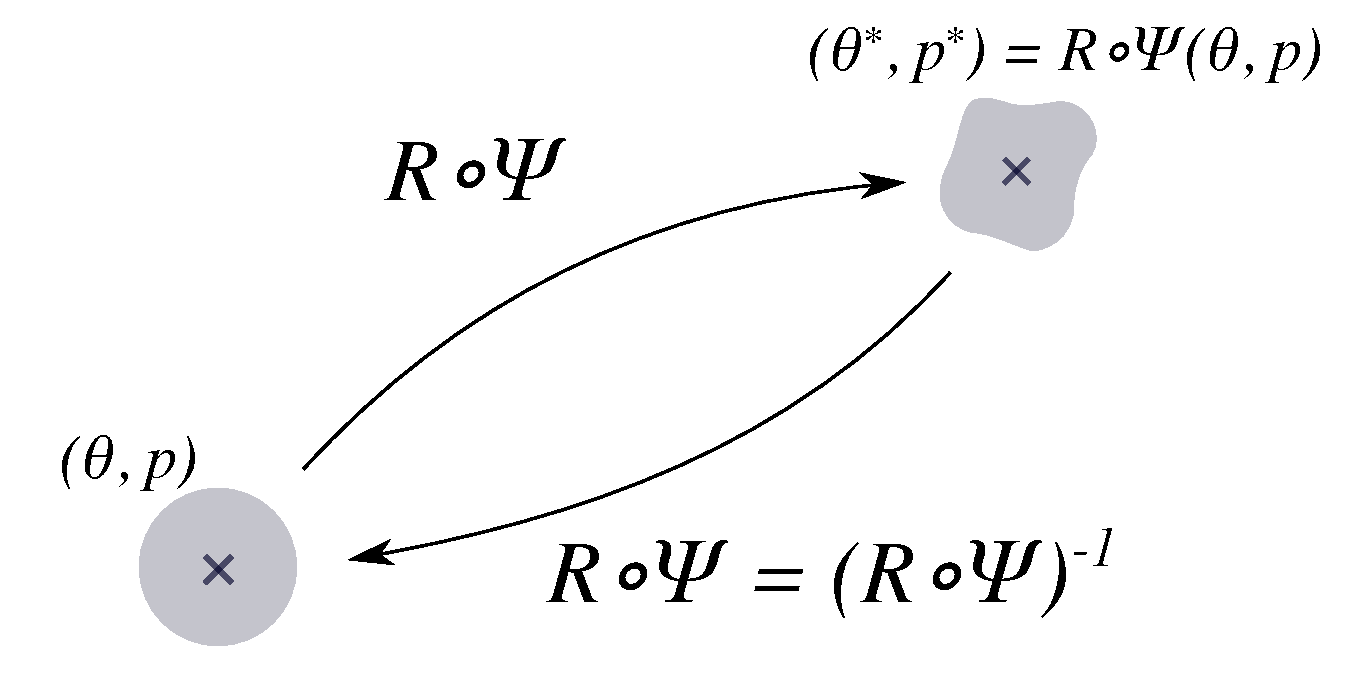
\includegraphics[height=.45\textheight]{Figure/reversible_map}
	\end{figure}
}

\frame{
	\frametitle{Geometric / structure-preserving numerical integration}
	\begin{itemize}
	\item In practice, Hamiltonian dynamics must be numerically approximated.
	\item \textit{Integrator} refers to an algorithm for approximating solutions of ODEs.
	\item For an approximate dynamics to remain a valid proposal mechanism, the integrator must preserve reversibility (and volume-preservation).
	\item To approximate the evolution from time $t$ to $t + \stepsize$ of dynamics
		\begin{itemizedEquation*}
		\frac{\diff \bposition}{\diff t} 
			= m^{-1} \bmomentum, \quad
		\frac{\diff \bmomentum}{\diff t} 
			= - \nabla U(\bposition),
		\end{itemizedEquation*}
		the \textit{leapfrog} (or \textit{velocity Verlet}) method carries out the updates
		\begin{itemizedEquation*}
		\arraycolsep=2pt
		\def\arraystretch{1.75}
		\begin{array}{ccccc}
		\bmomentum_{t + \stepsize / 2}
			&=& \bmomentum_t 
			&-& \displaystyle \frac{\stepsize}{2} \nabla U(\bposition_t) \\
		\bposition_{t + \stepsize}
			&=& \bposition_t
			&+& \stepsize \, m^{-1} \bmomentum_{t + \stepsize / 2} \\
		\bmomentum_{t + \stepsize}
			&=& \bmomentum_{t + \stepsize / 2}
			&-& \displaystyle \frac{\stepsize}{2} \nabla U(\bposition_{t + \stepsize}).
		\end{array}
		\end{itemizedEquation*}
	\item Map $\solutionOp_{\stepsize}^\pathlen$ induced by $\pathlen(\tau) = \lfloor \tau / \stepsize \rfloor$ steps of the leapfrog updates approximate the exact evolution from time $t = 0$ to $t = \integrationTime$. 
	\end{itemize}
}

\frame{
	\frametitle{High acceptance rate of HMC proposals}
	\begin{itemize}
	\item If we could solve Hamiltonian dynamics exactly, then HMC proposals would have $100\%$ (!) acceptance rates.
	\item In essence, this is because the target $\pi(\cdot, \cdot)$ is an \textit{invariant} distribution of the dynamics --- if $(\bposition, \bmomentum) \sim \pi(\cdot, \cdot)$, then $\solutionOp_t(\bposition, \bmomentum) \sim \pi(\cdot, \cdot)$ for all $t$.
	\item With numerical approximation, acceptance rate of HMC proposals  converges to 1 as $\stepsize \to 0$ for a fixed $\tau$ and $\pathlen(\tau) = \lfloor \tau / \stepsize \rfloor$.
		% TODO : later provide a more quantitative discussion of the error as a function of stepsize.
	\end{itemize}
}

\frame{
	\frametitle{Acceptance probability of proposals via reversible map}
	\begin{itemize}
	\item For a general reversible map $\solutionOp$, the correct acceptance probability of a proposal $(\bposition^*, \bmomentum^*) = \solutionOp(\bposition, \bmomentum)$ is given by 
		\begin{itemizedEquation*}
		\min \! \left\{
			1, \, \frac{
				\pi(\bposition^*, \bmomentum^*) \left| \Diff \solutionOp(\bposition, \bmomentum) \right|
			}{
				\pi(\bposition, \bmomentum)}
		\right\}
		\end{itemizedEquation*}
		\vspace{-.5\baselineskip}
		\begin{itemize}
		\item To see why the Jacobian is needed, recall that the density of a transformed variables $(\bposition^*, \bmomentum^*) = \solutionOp(\bposition, \bmomentum)$ is given as
			\begin{itemizedEquation*}
			\pi_{\Position^*, \, \Momentum^*}(\bposition^*, \bmomentum^*) 
				= \pi_{\Position, \, \Momentum}(\bposition, \bmomentum) \left| \Diff \solutionOp(\bposition, \bmomentum) \right|^{-1}.
			\end{itemizedEquation*}
		\end{itemize}
	\item Hamiltonian dynamics and its leapfrog approximation are both volume-preserving, meaning $\left| \Diff \solutionOp_{\integrationTime} \right| = \left| \Diff \solutionOp_{\stepsize}^\pathlen \right| = 1$.
	\item Hence, the acceptance probability of an HMC proposal is
		\begin{itemizedEquation*}
		\min \! \left\{
			1, \, \frac{
				\pi(\bposition^*, \bmomentum^*)
			}{
				\pi(\bposition, \bmomentum)}
		\right\}
			= \min \! \left\{
				1, \, \exp\!\big( H(\bposition, \bmomentum) - H(\bposition^*, \bmomentum^*) \big)
			\right\}.
		\end{itemizedEquation*}
	\end{itemize}
}

\frame{
	\frametitle{Energy-conservation property for high acceptance rate}
	\begin{itemize}
	\item Hamiltonian dynamics is \textit{energy-conserving}, meaning the Hamiltonian remains constant along its trajectory $(\bposition(t), \bmomentum(t))$:
		\begin{itemizedEquation*}
		H(\bposition(t), \bmomentum(t)) 
			= H(\bposition(0), \bmomentum(0))
			\ \text{ for all } \ t.
		\end{itemizedEquation*}
	\item With the leapfrog approximation for a fixed $\integrationTime$,  the error is
		\begin{itemizedEquation*}
		\Delta H
			= H(\bposition_{L \stepsize}, \bmomentum_{L \stepsize})
				- H(\bposition_{0}, \bmomentum_{0})
			= O(\stepsize^2).
		\end{itemizedEquation*}
	\item Metropolis proposals in general satisfies, as $\Delta H \to 0$,
		\begin{itemizedEquation*}
		\mathbb{E}\left[ \Delta H \right]
			\approx \frac{1}{2} \, \mathbb{E}\left[ \Delta H^2 \right]
		\end{itemizedEquation*}
		% Note: we have an actual bound $E[\Delta H] \leq E[\Delta H^2]$ for a reversible dynamics-based proposal.
		% Note: the above relation holds for any Metropolis type algorithm
	\item HMC proposals thus satisfies $\mathbb{E}[\Delta H] = O(\stepsize^{\textcolor{lava}{4}})$ as $\stepsize \to 0$.
	\item e.g.\ HMC generates one effective sample from $\nparam$-dimensional Gaussians with the cost of
		\begin{itemizedEquation*}
		\nparam^{1 / 4} \times \text{(cost of likelihood \& gradient evaluation)}.
		\end{itemizedEquation*}
	\end{itemize}
}


\end{document}